\section{Aerodynamic Characteristics}

UH-60 aerodynamic characteristics are given in \cite{NASA-CR-166309}.

\subsection{Fuselage Aerodynamic Characteristics}

\csvreader[
  no head,
  longtable=cccc,
  table head=
    \toprule
    $\alpha$ & $D/q$ & $L/q$ & $M_Y/q$ \\
    {[deg]} & {[m\textsuperscript{2}]} & {[m\textsuperscript{2}]} & {[m\textsuperscript{3}]} \\ \midrule
    \endfirsthead
    $\alpha$ & $D/q$ & $L/q$ & $M_Y/q$ \\
    {[deg]} & {[m\textsuperscript{2}]} & {[m\textsuperscript{2}]} & {[m\textsuperscript{3}]} \\ \midrule
    \endhead,
  before first line={},
  late after line=\\,
  late after last line=\\ \bottomrule \caption{Fuselage aerodynamic characteristics due to angle of attack \cite{NASA-CR-166309}},
  before reading={},
  after reading={}
]
{csv/uh60_aero_fuselage.csv}
{1=\colaoa,2=\colcx,3=\colcy,4=\colcz,5=\colcl,6=\colcm,7=\colcn,8=\coldcx}
{\colaoa & \colcx & \colcz & \colcm}

\clearpage

\csvreader[
  no head,
  longtable=cccc,
  table head=
    \toprule
    $\beta$ & $Y/q$ & $M_X/q$ & $M_Z/q$ \\
    {[deg]} & {[m\textsuperscript{2}]} & {[m\textsuperscript{3}]} & {[m\textsuperscript{3}]} \\ \midrule
    \endfirsthead
    $\beta$ & $Y/q$ & $M_X/q$ & $M_Z/q$ \\
    {[deg]} & {[m\textsuperscript{2}]} & {[m\textsuperscript{3}]} & {[m\textsuperscript{3}]} \\ \midrule
    \endhead,
  before first line={},
  late after line=\\,
  late after last line=\\ \bottomrule \caption{Fuselage aerodynamic characteristics due to sideslip \cite{NASA-CR-166309}},
  before reading={},
  after reading={}
]
{csv/uh60_aero_fuselage.csv}
{1=\colbeta,2=\colcx,3=\colcy,4=\colcz,5=\colcl,6=\colcm,7=\colcn,8=\coldcx}
{\colbeta & \colcy & \colcl & \colcn}

\begin{figure}
  \centering
  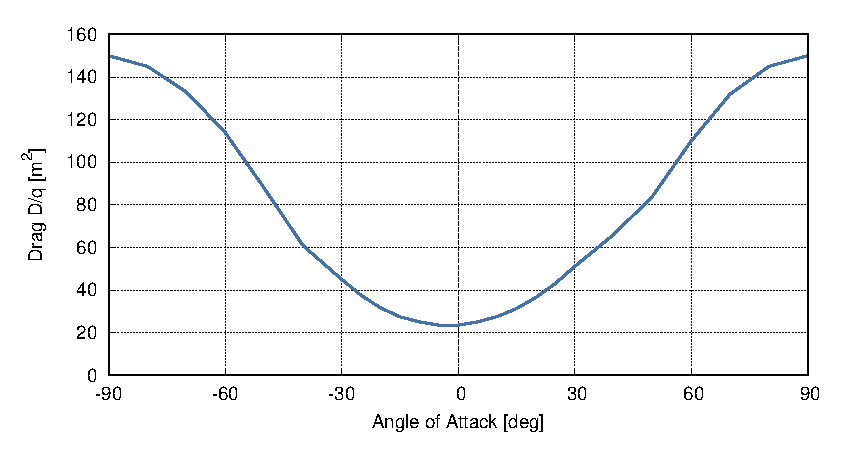
\includegraphics[width=140mm]{eps/uh60_fuselage_alpha_cx.eps}
  \caption{Fuselage drag due to angle of attack \cite{NASA-CR-166309}}
\end{figure}

\begin{figure}
  \centering
  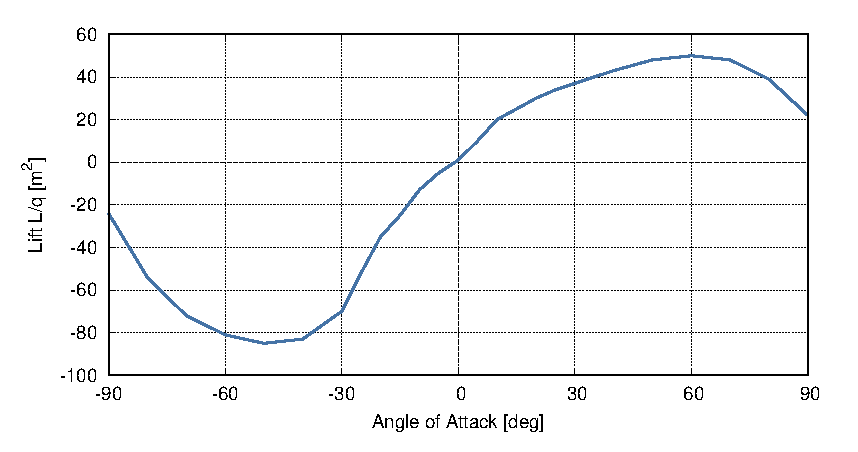
\includegraphics[width=140mm]{eps/uh60_fuselage_alpha_cz.eps}
  \caption{Fuselage lift due to angle of attack \cite{NASA-CR-166309}}
\end{figure}

\begin{figure}
  \centering
  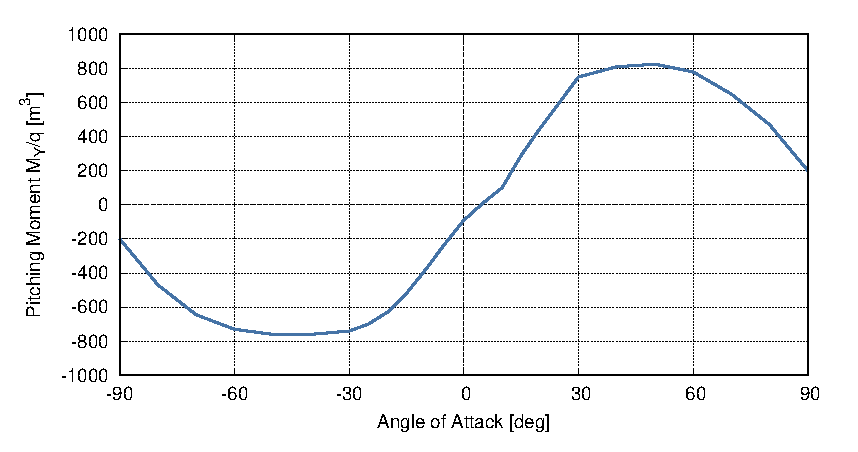
\includegraphics[width=140mm]{eps/uh60_fuselage_alpha_cm.eps}
  \caption{Fuselage pitching moment due to angle of attack \cite{NASA-CR-166309}}
\end{figure}

\begin{figure}
  \centering
  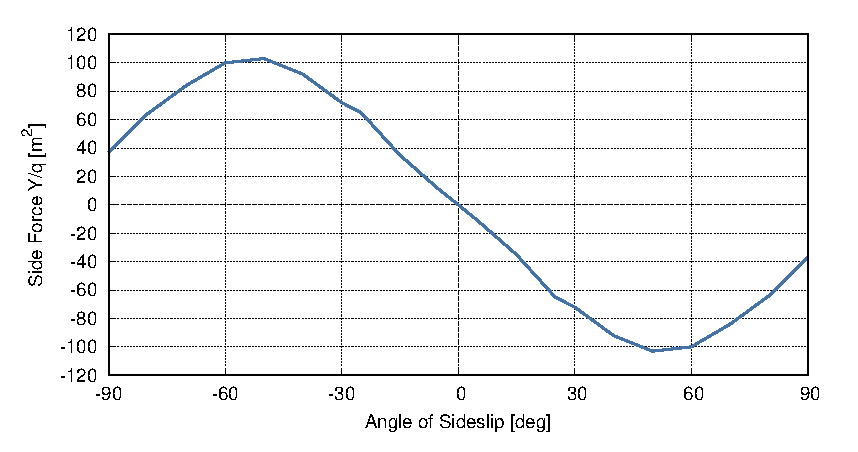
\includegraphics[width=140mm]{eps/uh60_fuselage_beta_cy.eps}
  \caption{Fuselage side force due to sideslip \cite{NASA-CR-166309}}
\end{figure}

\begin{figure}
  \centering
  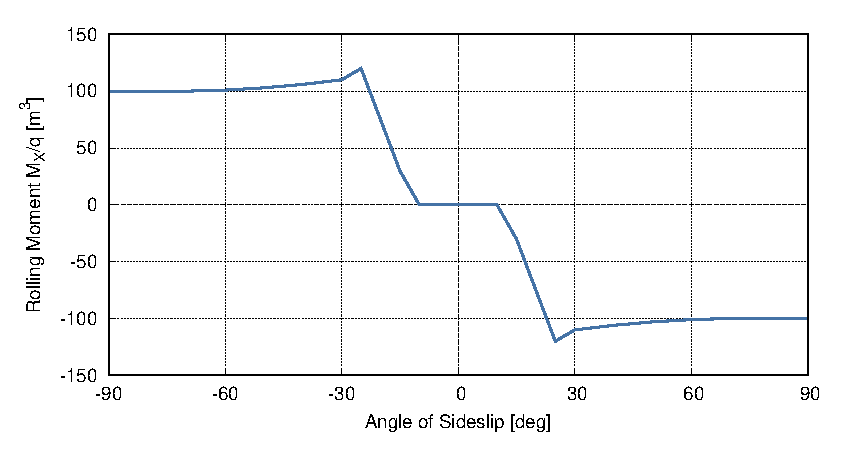
\includegraphics[width=140mm]{eps/uh60_fuselage_beta_cl.eps}
  \caption{Fuselage rolling moment due to sideslip \cite{NASA-CR-166309}}
\end{figure}

\begin{figure}
  \centering
  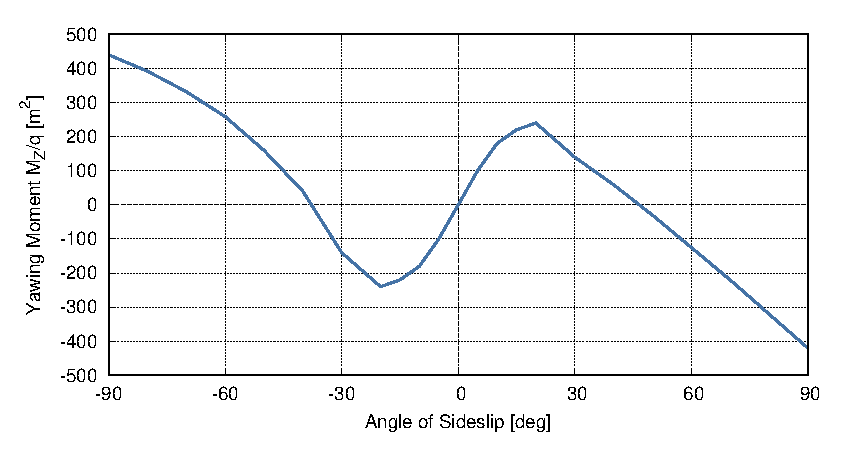
\includegraphics[width=140mm]{eps/uh60_fuselage_beta_cn.eps}
  \caption{Fuselage yawing moment due to sideslip \cite{NASA-CR-166309}}
\end{figure}


\clearpage
\subsection{Fuselage Incremental Aerodynamic Characteristics}

\csvreader[
  no head,
  longtable=cccc,
  table head=
    \toprule
    $\beta$ & $\Delta D/q$ & $\Delta L/q$ & $\Delta M_Y/q$ \\
    {[deg]} & {[m\textsuperscript{2}]} & {[m\textsuperscript{2}]} & {[m\textsuperscript{3}]} \\ \midrule
    \endfirsthead
    $\beta$ & $\Delta D/q$ & $\Delta L/q$ & $\Delta M_Y/q$ \\
    {[deg]} & {[m\textsuperscript{2}]} & {[m\textsuperscript{2}]} & {[m\textsuperscript{3}]} \\ \midrule
    \endhead,
  before first line={},
  late after line=\\,
  late after last line=\\ \bottomrule \caption{Fuselage incremental aerodynamic characteristics \cite{NASA-CR-166309}},
  before reading={},
  after reading={}
]
{csv/uh60_aero_fuselage_3.csv}
{1=\colbeta,2=\coldcx,3=\coldcz,4=\coldcm}
{\colbeta & \coldcx & \coldcz & \coldcm}

\begin{figure}
  \centering
  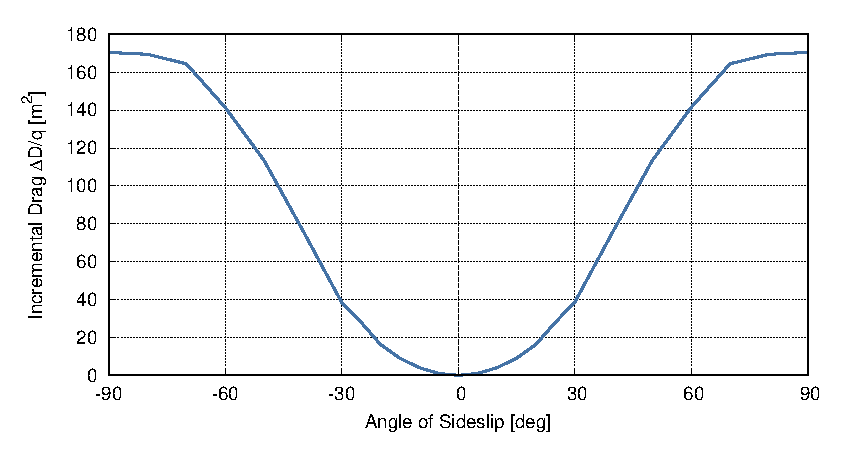
\includegraphics[width=140mm]{eps/uh60_fuselage_beta_dcx.eps}
  \caption{Fuselage incremental drag due to sideslip \cite{NASA-CR-166309}}
\end{figure}

\begin{figure}
  \centering
  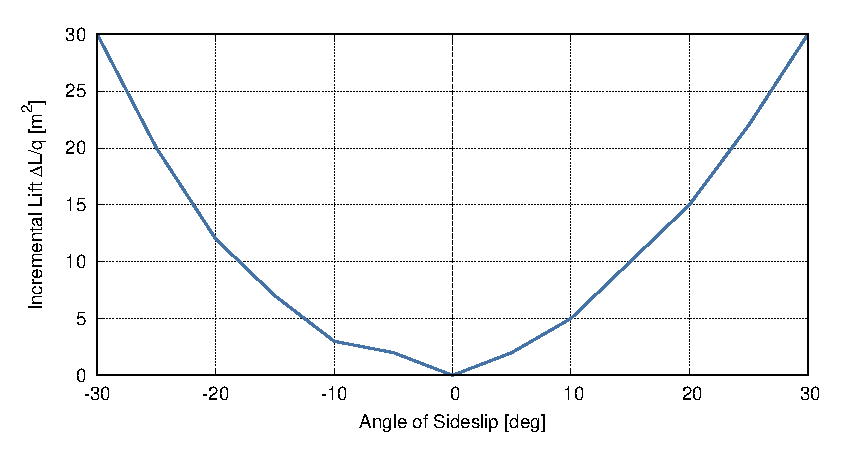
\includegraphics[width=140mm]{eps/uh60_fuselage_beta_dcz.eps}
  \caption{Fuselage incremental lift due to sideslip \cite{NASA-CR-166309}}
\end{figure}

\begin{figure}
  \centering
  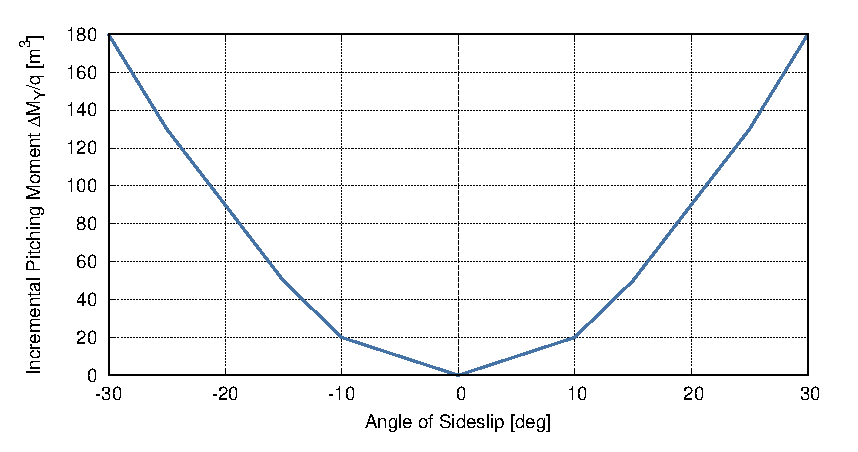
\includegraphics[width=140mm]{eps/uh60_fuselage_beta_dcm.eps}
  \caption{Fuselage incremental pitching moment due to sideslip \cite{NASA-CR-166309}}
\end{figure}

\clearpage
\subsection{Horizontal Tail Aerodynamic Coefficients}

Horizontal tail reference area: 4.18 [m\textsuperscript{2}]

\csvreader[
  no head,
  longtable=ccc,
  table head=
    \toprule
    $\alpha$ & $C_{X,h}$ & $C_{Z,h}$ \\
    {[deg]} & {[-]} & {[-]} \\ \midrule
    \endfirsthead
    $\alpha$ & $C_{X,h}$ & $C_{Z,h}$ \\
    {[deg]} & {[-]} & {[-]} \\ \midrule
    \endhead,
  before first line={},
  late after line=\\,
  late after last line=\\ \bottomrule \caption{Horizontal tail aerodynamic coefficients \cite{NASA-CR-166309}},
  before reading={},
  after reading={}
]
{csv/uh60_aero_empennage.csv}
{1=\colaoa,2=\colhcx,3=\colhcz,4=\colvcx,5=\colvcy}
{\colaoa & \colhcx & \colhcz}

\begin{figure}
  \centering
  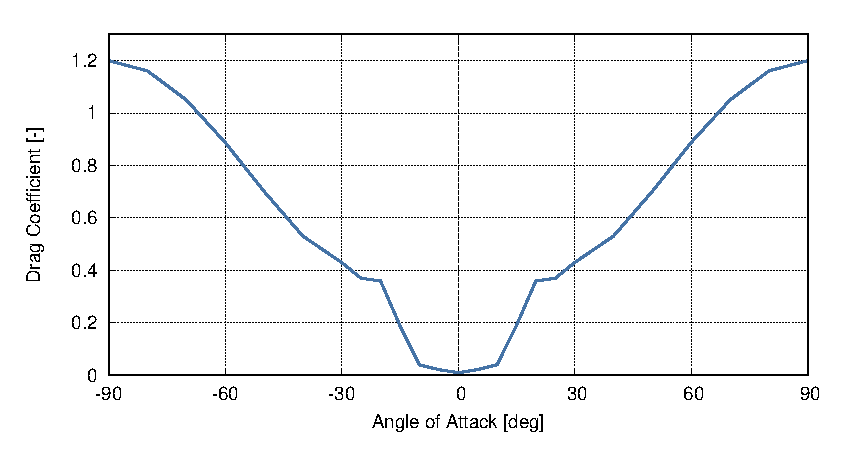
\includegraphics[width=140mm]{eps/uh60_stab_h_cx.eps}
  \caption{Horizontal tail drag coefficient due to angle of attack \cite{NASA-CR-166309}}
\end{figure}

\begin{figure}
  \centering
  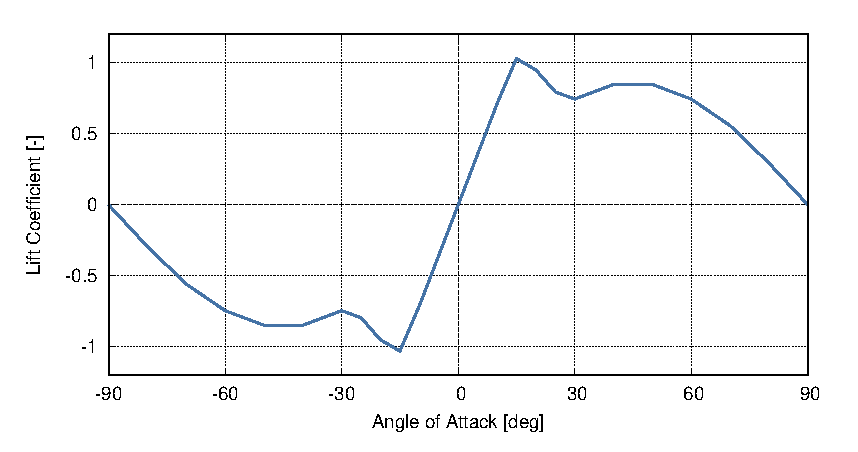
\includegraphics[width=140mm]{eps/uh60_stab_h_cz.eps}
  \caption{Horizontal tail lift coefficient due to angle of attack \cite{NASA-CR-166309}}
\end{figure}

\clearpage
\subsection{Vertical Tail Aerodynamic Coefficients}

Vertical tail reference area: 3.00 [m\textsuperscript{2}]

\csvreader[
  no head,
  longtable=ccc,
  table head=
    \toprule
    $\beta$ & $C_{X,v}$ & $C_{Y,v}$ \\
    {[deg]} & {[-]} & {[-]} \\ \midrule
    \endfirsthead
    $\beta$ & $C_{X,v}$ & $C_{Y,v}$ \\
    {[deg]} & {[-]} & {[-]} \\ \midrule
    \endhead,
  before first line={},
  late after line=\\,
  late after last line=\\ \bottomrule \caption{Vertical tail aerodynamic coefficients \cite{NASA-CR-166309}},
  before reading={},
  after reading={}
]
{csv/uh60_aero_empennage.csv}
{1=\colbeta,2=\colhcx,3=\colhcz,4=\colvcx,5=\colvcy}
{\colbeta & \colvcx & \colvcy}

\begin{figure}
  \centering
  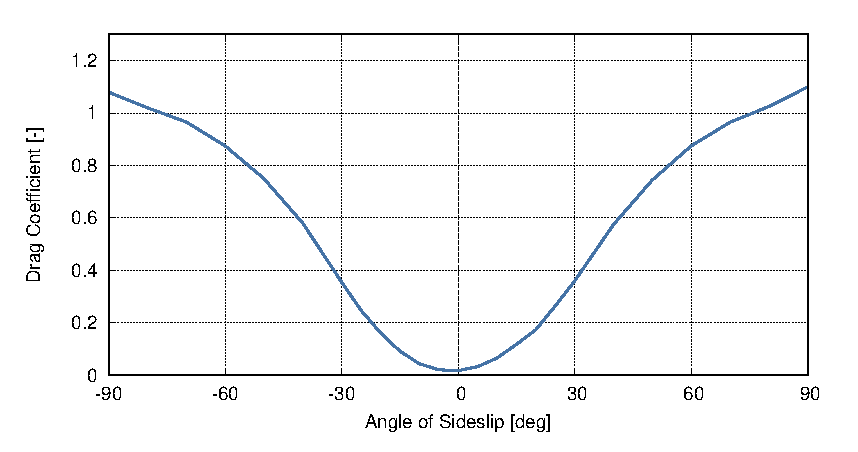
\includegraphics[width=140mm]{eps/uh60_stab_v_cx.eps}
  \caption{Vertical tail drag coefficient due to sideslip \cite{NASA-CR-166309}}
\end{figure}

\begin{figure}
  \centering
  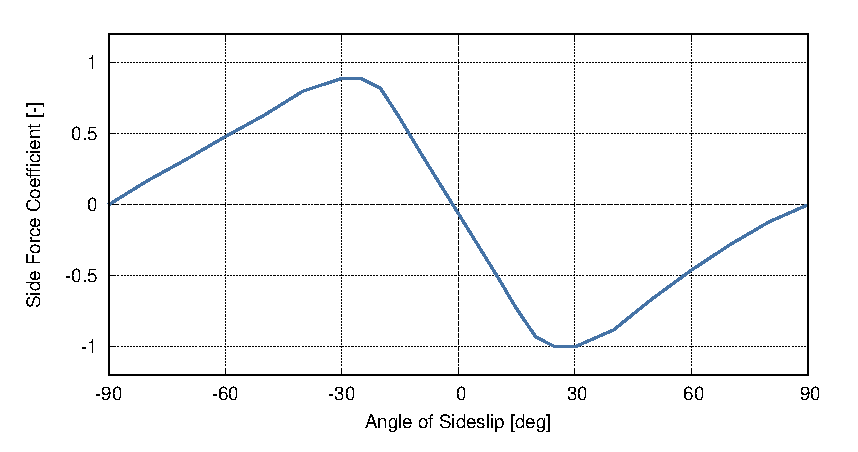
\includegraphics[width=140mm]{eps/uh60_stab_v_cy.eps}
  \caption{Vertical tail side force coefficient due to sideslip \cite{NASA-CR-166309}}
\end{figure}
